\subsection{Теорема Клини.}

Продолжаем доказывать, но уже в правую сторону

\begin{enumerate}
    \item[2.] $Aut \subset Reg$

    $L \in Aut: A$ - ДКА для $L$.

    $Q = \{1,\ldots, n\}$

    $\xi_{ijk}$ - слова, такие, что $i,j$ и переход по вершинам номера которых меньше $k$.

    Построим $n^3$ таких регулярных выражений таким образом:
    $$\xi_{ij (k+1)} = \xi_{ijk} | \xi_{i(k+1)k}(\xi_{(k+1) (k+1) k})^* \xi_{(k+1)jk}$$
    (Случай $k=0$ тривиален, используем его как за базу)
    
    Откуда наше регулярное: $\varphi = \xi_{s t_1n}|\xi_{st_2n}|\ldots$
    
\end{enumerate}

\hfill Q.E.D.

\subsection{Нерегулярность}

Язык правильных скобочных последовательностей не является регулярным языком.

\textbf{Доказательство:}

Пусть ПСП $\in Reg$, $A$ - ДКА для ПСП. Пусть $n$ число сост. $A$.

Скормим ему $(,((,(((,((((,\ldots$: до их размера $n+1$. По принципу Дирихле у нас будут 2 конечных состояния у этих строк, которые совпадут. Пусть $q_i = q_j  = u$. Тогда посмотрим на строки $x= (^i)^i$ и $y = (^j)^i$. Заметим, что они придут в конечное одно состояние. Причем $x$---ПСП, $y$---нет. Противоречие.

\hfill Q.E.D.

\deff{Нерегулярный язык} - это формальный язык, который не может быть описан ни одним из вышеупомянутых способов (регулярным выражением, конечным автоматом или регулярной грамматикой).

Примеры:

$L = \{a^n b^n | n \geq 0\}$

$L = \{w w^R | w \in \{a, b\}* \}$ - \deff{язые палиндромов}

\thmm{Теорема (Лемма о разрастании/накачке)}

$L$ - регулярный язык. Тогда:

$\exists n > 0: \forall w:w \in L, |w|\geq n , \exists x,y,z : w =xyz$, такие, что $y \neq \varepsilon, |xy|\leq n, \forall k\geq 0, xy^kz\in L$

\textbf{Доказательство:}

Пусть $L$ - регулярный язык, тогда существует ДКА для $L$. Пусть $n$ - число состояний автомата $A$. $\forall w \in L, |w| \geq n$.

\begin{center}
    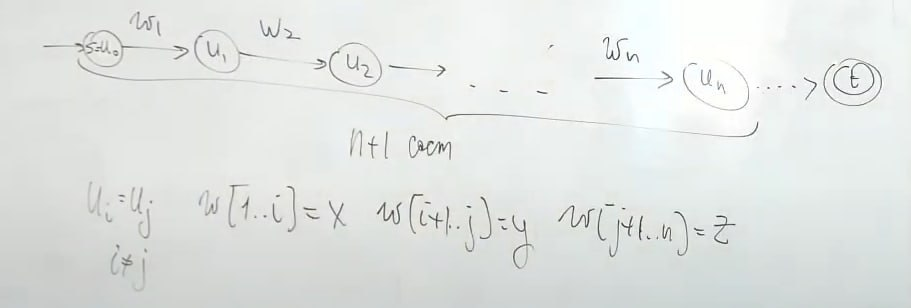
\includegraphics[width = 12cm]{assets/9_2_1.jpg}
\end{center}

Возьму первые $n+1$ состояний. По принципу Дирихле будут совпадающие(мы нашли цикл). Возьмем за $y$ - данный цикл, $x$ - всего до него $z$ - все после. Откуда верность утверждения тривиальна.

\textbf{Следствие.} Не выполнено данное утверждение $\Rightarrow$ не регулярный.

У любого языка есть минимальный автомат (линейная алгебра передает привет).

\deff{Алгоритм минимизации автомата.}

Д.К.А $A$. $u$ и $v$ назовем \deff{различимыми} строкой $s$: если из $u$ можно перейти в какой-то $x$, а из $v$ можно перейти в $y$ с помощью слова $s$, причем либо $x$, либо $y$ терменальная.

Назовем $a \mytilde b$,  если $a$ и $b$ не различимы никакой строкой. Очевидно $\mytilde$ это отношение эквивалентности, откуда можно разбить на классы эквивалентности.

\thmm{Лемма:} $u \mytilde v \Rightarrow \delta(u,c) \mytilde \delta(v,c)$. Очевидно.

Алгоритм: Обозначим $D_k = \{(u,v) | u,w \text{ различимы } s,|s|\leq k\}$
$$D_0 = \{(u,v) | u\in T \oplus v \in T \}$$
$$D_k = \{(u,v) | (u,v) \in D_{k-1} ||\exists c \in \Sigma:(\delta(u,c),\delta(v,c))\in D_{k-1}\}$$
Тогда у нас вот примерно такой алгоритм поиска  эквивалентных:

\begin{lstlisting}[mathescape]
    \\$\text{Положим D0 в Q, D0 в D, Q - очередь}$
    while not Q.empty():
        (u,v) = Q.pop()
        for c in Sigma:
            for a in In[u][c]
                for b in In[v][c]:
                    if(a,b) not in D:
                        q.push(a,b)
                        D.add(a,b)
\end{lstlisting}

То есть мы умеем искать пары эквивалентных.

\thmm{Теорема.} $A$ - ДКА для $L$ не содержит эквивалентных и любое состояние достидимо из $s$ тогда:
\begin{enumerate}
    \item $A$ - минимальный.
    \item $A'$ - ДКА для $L$. $|Q'|=|Q|$, тогда $A'$ изоморфно $A$.
\end{enumerate}

\textbf{Доказательство:}

Пусть есть автомат с меньшим количеством вершин. Назовем его $B$. Посмотрим на автомат Объединения. Есть два стартовых состояния. Забьем на них пока что. Давайте на получившимся автомате запустим автомат из теоремы. Что мы знаем? Стартовые состояния, очевидно, оказались эквивалентными. Возьмем какую-нибудь вершину из $A$(назовем ее $u$) и придем в нее через стартовую, повторяя эти действия во втором автомате, то по лемме они придут в эквивалентные состояния. Так как у нас достижимо из стартовой каждое состояние в $A$, то у меня будет $n$ пар эквивалентностей $A$ и $B$, откуда, тк справа вершин $<n$ или по-другому $\leq n-1$, то по принципу Дирихле у какие-то 2 состояния из A эквивалентны одному из $B$, а так как это эквивалентность, то они сами экивалентны друг другу, что противоречит условию. Откуда, B не может быть меньшего размера. Если $B$ такого же размера, как и $A$, то мы показали, что у нас образуются пары экивалентных.

\hfill Q.E.D.


